% TODO_ The following notions must have been introduced before:
% - The trace invariant (but not the message invariant)

\chapter{Case study}

Now that we have presented our methodology and its implementation in the Reusable Verification Library, we will apply it to a protocol to showcase its use. 
In this chapter, our goal is to show that the library is now able to verify a protocol whose security properties rely on the frequent deletion of sensitive data.

\todo{Write the outline}

\section{Choosing a protocol to verify}
\label{sec:choosing-a-protocol-to-verify}

First, we decide on a protocol to verify.
We take several criteria into account, which we list here in order of importance.
First, the protocol must use ephemeral keys that exist only for a short time before being deleted, to satisfy some strong security property.
Second, we want the protocol to be simple enough to be implemented and verified in a reasonable amount of time. As we only aim to showcase the use of our extended verification library, there is no need to use a state-of-the-art security protocol.
And third, we want to derive our protocol from an existing one, to show that our library can verify real-world protocols, and not only toy examples.

In this section, we start by presenting the Diffie-Hellman ratchet, a protocol that checks almost all of our criteria. 
We continue by introducing a necessary phase of key agreement to obtain the prior knowledge required by such protocol.
Finally, we present our final choice of protocol, a modified version of the Diffie-Hellman ratchet, and explain why we made this choice.

\subsection{Ratcheting protocols}
\label{sec:ratcheting-protocols}
% DH Ratchet, Signal

We have already mentioned the Signal protocol in the previous chapters, which is based on the Double Ratchet algorithm.
Signal is a state-of-the-art protocol, whose verification of a Go implementation has, to the best of our knowledge, never been attempted.
However, we do not consider that we have sufficient time to verify such a complex protocol implementation in the scope of this thesis.
Optimally, we would like to verify a protocol implementation that is simpler than Signal, but uses the same principles of ephemeral keys and ratcheting to achieve comparable security properties.

Such a protocol exists and has already been introduced in section \ref{sec:diffie-hellman-ratchet}: the Diffie-Hellman (DH) Ratchet.
Recall that the DH Ratchet is the core component of the Signal protocol. Participants frequently exchange their Diffie-Hellman public keys and use them to obtain a shared secret that is used to derive new ephemeral keys to encrypt their messages.
The DH Ratchet aims to provide both forward secrecy and post-compromise security, which are the same security properties that Signal aims to achieve.
If the DH Ratchet can provide the same guarantees as the more complex Signal protocol, it is because the DH Ratchet uses a simpler communication model, where participants alternate sending and receiving messages.
In Signal, the protocol has to cope with a participant sending multiple messages in a row, as well as out-of-order and lost messages.

While the DH Ratchet now appears to be a good candidate for our case study, we have to handle the fact that it requires some prior knowledge, as it was shown in Figure \ref{fig:dh-ratchet}.
We need to provide the initiator and responder with a shared secret $K_0$, which will be the initial key of their key chain.
Additionally, we need to provide the initiator with the public key $g^{y_0}$ of the responder, where $y_0$ is the private of the responder.
We cannot use the DH Ratchet without this prior knowledge, which requires us to add an initial key agreement to the protocol.

\subsection{Initial key agreement}
\label{sec:initial-key-agreement}
% X3DH, WireGuard noise's Handshake

Similarly to the Diffie-Hellman Ratchet, the Signal protocol starts with an initial key agreement before running the Double Ratchet algorithm.
Signal uses the X3DH key agreement protocol, which is a state-of-the-art protocol that provides forward secrecy and cryptographic deniability.
Additionally, X3DH is specifically designed to work asynchronously when one user is offline.
Because X3DH is a complex protocol that would require significant time to implement and verify, and because we do not necessarily need all of its strong security properties, we are going to use a simpler protocol.

We use the fact that the WireGuard protocol has already been implemented and verified with the Reusable Verification Library.
WireGuard starts with a handshake based on a Diffie-Hellman key exchange, called the \emph{Noise IKpsk2} handshake from the Noise protocol. This handshake establishes symmetric keys between the initiator and responder, which is the first part of the prior knowledge required by the DH Ratchet.
\todo{Should I mention the security properties of the handshake (strong/weak forward secrecy)?}

Then, it is easy to add a communication round between the initiator and responder, in which the responder computes a Diffie-Hellman key pair and sends its public key to the initiator, authenticated with the symmetric key established by the handshake.\todo{This is not really a communication “round” because there is just one message, no response.}
Therefore, if we combine the IKpsk2 handshake with this additional communication round, we obtain the prior knowledge required by the DH Ratchet.
At this point, we have a ratcheting protocol that satisfies the three criteria introduced at the beginning of this section. However, we made an additional modification to simplify the verification process.

\subsection{Chosen protocol}
\label{sec:chosen-protocol}

As shown in Figure \ref{fig:dh-ratchet}, when the initiator sends a message encrypted by a key $K_1$ to the responder together with its new public key $g^{x_1}$, the responder uses this public key $g^{x_1}$ to compute the shared secret $K_1$ and decrypt the message.
Typically, the public key $g^{x_1}$ is sent in the associated data of the AEAD encrypted message, so its integrity is protected, but it remains publicly readable so the responder can immediately access it to compute $K_1$.

In the existing methodology and its current implementation, the Reusable Verification Library, the message comes with a ghost \emph{message invariant}. It is a property, part of the trace invariant, about the content of the message used for verification purposes. Upon encrypting the message to send, the initiator has to prove this message invariant, and upon receiving and decrypting the message, the responder can either assume the message invariant or know that corruption has occurred.
In our case, for the first message sent by the initiator on Figure \ref{fig:dh-ratchet}, the message invariant would contain information about the public key $g^{x_1}$. In particular, it would contain that $g^{x_1}$ is an exponential with base generator $g$ and exponent $x_1$, where $x_1$ is a nonce readable by the initiator.
This information can then be used for verification purposes on the responder side, notably to know that $g^{x_1y_0}$ is a Diffie-Hellman shared secret.

However, in our case, it is a problem that the message invariant is obtained only \emph{after} decryption of the message because we would need to know that $g^{x_1y_0}$ is a shared secret \emph{before} decryption to be able to decrypt the message.
Indeed, the decryption function requires us to prove that $K_1$ is a valid AEAD decryption key, which we can only know if we know that $g^{x_1y_0}$ is a shared secret.

This is why we decided to slightly modify the DH Ratchet protocol to make it verifiable with our existing methodology and library.
We present our modified protocol in Figure \ref{fig:dh-ratchet-modified}, and our new first communication round (running after the IKpsk2 handshake) in Figure \ref{fig:dh-ratchet-modified-first}.
For the sake of readability, we will now refer in all future parts to our modified DH Ratchet protocol as the \emph{ratcheting protocol}. Additionally, we will refer to the entire protocol that we verify, e.g. the IKpsk2 handshake followed by the first communication round and the ratcheting protocol, as the \emph{full ratcheting protocol}.

\begin{figure}
    \centering
    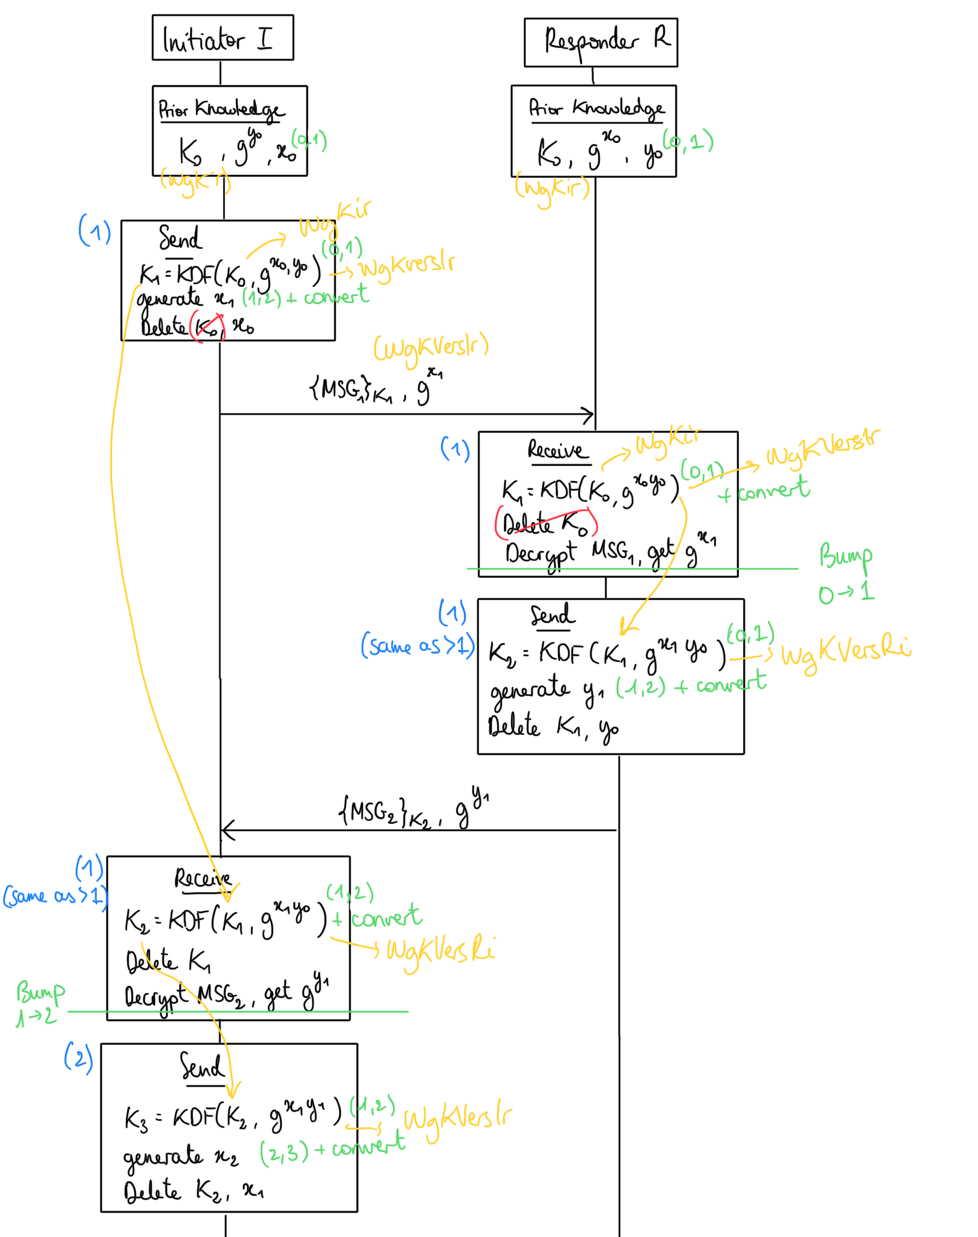
\includegraphics[width=0.9\textwidth]{figures/DH-ratchet-modified.png}
    \caption{Our \emph{ratcheting protocol}, a modified protocol based on the Diffie-Hellman Ratchet.}
    \label{fig:dh-ratchet-modified}
\end{figure}

\begin{figure}
    \centering
    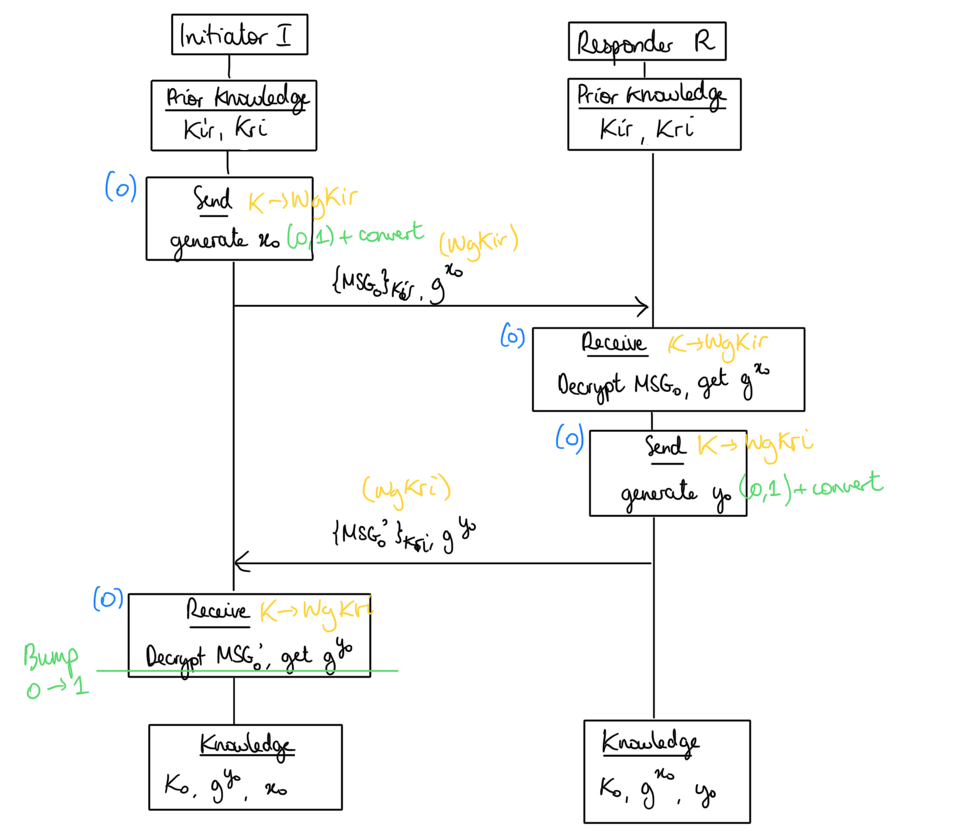
\includegraphics[width=0.9\textwidth]{figures/DH-ratchet-modified-first.png}
    \caption{First communication round after the handshake.}
    \label{fig:dh-ratchet-modified-first}
\end{figure}
\todo{Change the figures \ref{fig:dh-ratchet-modified} and \ref{fig:dh-ratchet-modified-first} to use cleaner ones, and modify the caption to explain the figures more in detail}

The intuition behind the ratcheting protocol is that we replicate the DH Ratchet protocol, but instead of using the just-received public key to compute the shared secret used in the message decryption, we use the public key received in the previous message.
This first requires us to modify the prior knowledge of the participants. Now, in addition to the initial shared secret $K_0$, both participants need to know the other's public key and their private key.
This is the purpose of the new first communication round shown in Figure \ref{fig:dh-ratchet-modified-first}. 
The initiator first sends its public key $g^{x_0}$ to the responder, authenticated with the symmetric key established by the handshake. Then, the responder replies with its authenticated public key $g^{y_0}$.

Coming back to the ratcheting protocol shown in Figure \ref{fig:dh-ratchet-modified}, when computing the first shared secret $K_1$, the initiator uses its private key $x_0$, whose associated public key $g^{x_0}$ is already known by the responder, from the first communication round.
This was not the case in the DH Ratchet protocol.
The first message sent by the initiator to the responder is otherwise the same as in the DH Ratchet protocol and contains the initiator's new authenticated public key $g^{x_1}$ in addition to the encrypted message.
Upon reception of this message by the responder, instead of using the public key $g^{x_1}$ to compute the shared secret $K_1$, the responder uses the previous public key $g^{x_0}$ received in the first communication round.
This allows the responder to obtain $K_1$, decrypt the message, and obtain the associated message invariant containing information about the new public key $g^{x_1}$.
Then, $g^{x_1}$ is used just after by the responder to compute the next shared secret $K_2$, which is used to encrypt the next message sent to the initiator.
The same observations can be made upon reception of the second message by the initiator, and all subsequent messages. 
\todo{Depending on how precise the final Figure \ref{fig:dh-ratchet-modified} is, I may need to explain the difference between the first message and the others: we do not delete the unversioned key $K_0$}

Ultimately, this ratcheting protocol is simpler to verify than the DH Ratchet and aims to provide similar security properties.
Intuitively, forward secrecy still holds because past communication keys are deleted and cryptographically not retrievable from long-term secrets and current communication keys.

Additionally, we show that post-compromise security still holds.
Considering a participant $p$ in a session $s$ and version $n$, we want to know how long the ratcheting protocol takes to heal. 
If $p$ is deriving a new communication key $K_n$, we look at the consequences if the attacker had compromised $p$ or its pair $p'$ in the past.
Recall that $p$ obtains their new key by computing $K_n := \text{KDF}(K_{n-1}, g^{xy})$, where $x$ and $y$ are private keys of $p$ and $p'$ respectively.
For a past compromise to impact this key $K_n$, the attacker would need to know $K_{n-1}$ and either $x$ or $y$. Indeed, $g^x$ and $g^y$ have been publicly exchanged, so the attacker only needs to know one private key to compute the shared secret $g^{xy}$.
Therefore, unless the attacker obtains $K_{n-1}$ and $x$ or $y$ between their creation and their deletion, the attacker cannot obtain $K_n$, meaning that the past compromise would not impact the future communication.
This shows that our ratcheting protocol satisfies post-compromise security.

For the sake of accuracy, we show that the difference between our protocol and the DH Ratchet protocol nevertheless has a slight impact on the exact property that our protocol satisfies.
Note that at this point, the reasoning above is valid for both the DH Ratchet protocol and our ratcheting protocol.
What differs between the two protocols is the amount of time between the creation of $K_{n-1}$, $x$ and $y$ and their deletion.
Intuitively, the longer this amount of time is, the more likely it is that the attacker obtains $K_{n-1}$ and $x$ or $y$ to derive $K_n$ and compromise future communication.
In our ratcheting protocol, we explained that $p$ uses the public key $g^y$ of $p'$ from the \emph{previous} communication round to compute the shared secret, instead of using the just-received one as in the DH Ratchet protocol.
This means that after $p'$ creates $y$, they will first send a message where $g^y$ is given as associated data, and in the next round $p'$ will use $y$ to compute the shared secret of the communication key $K_n$ to send their next message.
Because of this, $y$ still exists in the memory of $p'$ when they compute $K_n$ to encrypt the second message, whereas in the DH Ratchet protocol, $y$ would already be deleted and $K_n$ would be derived using a freshly generated private key.
\todo{This is not the case in the current figure showing the DH Ratchet. It should be changed to show the deletion of $x$ and $y$ in the receive function.}
In the end, our ratcheting protocol gives a slightly longer amount of time to the attacker to corrupt $p'$ to obtain $y$ before $K_n$ is computed, which would compromise all future communication.
% Our ratcheting protocol therefore verifies post-compromise security with a marginally weaker security property than the DH Ratchet protocol.

% Recall that post-compromise security \emph{via state} considers that some secret data remains known only by the participants after a compromise.
% With the DH Ratchet protocol, we assumed that the attacker compromised Alice's $K_n$ key (and state) \emph{after} she derived $K_{n+1}$, and this assumption was enough to obtain post-compromise security (section \ref{sec:security-properties}).
% However, this does not hold in this case.
% Suppose we have two participants Alice and Bob communicating, and that an attacker compromises Alice's state at the time when she computed $K_n$ after receiving a message.
% The attacker knows $K_n$, but also Alice's ephemeral private key $x_{n-1}$ and Bob's just-received public key $g^{y_{n-1}}$.
% The attacker can therefore compute $K_{n+1} = \text{KDF}(K_n, g^{x_{n-1}y_{n-1}})$ because it knows all the inputs of the KDF function, which was not the case with the DH Ratchet protocol.
% Unlike before, we have to assume that the attacker compromised Alice's $K_n$ key (and state) after she derived $K_{n+1}$ \emph{and} $K_{n+2}$.
% At this point, the attacker cannot obtain $K_{n+2}$ because they cannot have access to the new Diffie-Hellman shared secret.
% The protocol is therefore healed and achieves post-compromise security.

In the end, we have presented a full ratcheting protocol that draws its security properties from the frequent renewal of ephemeral keys. This protocol is mainly based on the Diffie-Hellman Ratchet protocol and has been slightly adapted to facilitate its verification. 
We will now present how we implemented and verified this protocol using our methodology and its implementation in the Reusable Verification Library. 

\section{Implementation and verification}
\label{sec:implementation-and-verification}

This section explains how we implemented and verified the full ratcheting protocol presented in the previous section.
We started the implementation on top of the existing WireGuard implementation, which already implements the IKpsk2 handshake.
The remaining work was to implement the first communication round and the ratcheting protocol.
In particular, the implementation work shed light on additional challenges related to the verification library. This section describes these challenges and how we solved them.

\todo{Write the outline}

\subsection{Ratcheting using a key derivation function}
\label{sec:ratcheting-using-a-key-derivation-function}

In section \ref{sec:creating-values-with-multiple-versions-for-ratcheting}, we explained how we designed our methodology to support key ratcheting, namely the derivation of a new key, versioned with a later version, from the previous one.
However, note that for now, we have not discussed the concrete specification and implementation of the ratcheting step. In particular, we have not discussed how we could obtain a $(v+1)$-versioned key from a $v$-versioned key.
% This is no coincidence, and we will explain why.

In practice, this ratcheting step is implemented by a key derivation function (KDF), taking the previous key as one of its inputs and returning the new key.
However, the precise KDF function used and the arguments it takes depend on the protocol. It is therefore not possible to provide a generic implementation of it in the library. This is why we have not discussed its implementation yet.
For our case study, the KDF function specification is given in Figure \ref{lst:kdf-ratchet}.

\begin{figure}
    \begin{gobra}
trusted
requires versionPerm > 0 && acc(guard(currentVersion), versionPerm)
ensures  acc(receipt(res, currentVersion), versionPerm)
func ComputeKDFRatchet(k []byte, dhss []byte, ghost currentVersion
    uint32, ghost versionPerm perm @*/) (res []byte) {
    // ...
}
    \end{gobra}
    \caption{Specification of the trusted \texttt{ComputeKDFRatchet} function, taking the previous key \texttt{k} and Diffie-Hellman shared secret \texttt{dhss} as input, and whose body computes the KDF result \texttt{res}. This protocol-specific KDF implementation is not part of the library but is written by the developer as part of the protocol. Preconditions and postconditions that are not relevant to the deletion mechanism have been omitted.}
    \label{lst:kdf-ratchet}
\end{figure}

\texttt{ComputeKDFRatchet} is the concrete implementation of our KDF function, and as the underlying KDF computations come from a non-verified library, we have to trust it.
As with any function creating a versioned value in our methodology, it consumes some permission fraction of \texttt{guard} predicate and returns the same amount of \texttt{receipt} for the created value. This ensures the soundness of our deletion mechanism.

Now, we want to define the secrecy label of the resulting KDF.
The secrecy label of a term is defined by a function \texttt{GetLabel} of the library. It can return a static label depending on the properties of the term, or a label depending on the arguments of the term when the term is a function of other terms. 
But first, to define a secrecy label for the KDF output, we need the library to \emph{know} about our KDF. While we defined it in the protocol, the KDF function needs to be specified on a term level in the library. We define it as follows:
\begin{gobra}
func KDFRatchet(Term, Term) Term
\end{gobra}
We additionally specify some of its properties, like injectivity, through axioms written in the library.
To then bridge the gap between the protocol and the library definitions, we add to the protocol's \texttt{ComputeKDFRatchet} function a postcondition ensuring that the KDF result corresponds to the byte representation of the library's KDF term.

Now that the library knows about our KDF, we can define its secrecy label.
Intuitively, the only rule about the secrecy of a KDF output is that it is at most as secure as knowing all of its inputs. Indeed, if you know all the inputs of a KDF, you can compute its output.
However, the KDF output is not necessarily as secure as its inputs. For example, a \emph{hash} function is a particular key derivation function that is generally used to obtain a public output from a secret input. 
Therefore, the secrecy label of the output of a KDF should be weaker or equal to the intersection of the secrecy labels of its inputs.

In our case, the output term \texttt{newk := KDFRatchet(k, dhss)} can have its secrecy label determined by the labels of the previous key \texttt{k} and the Diffie-Hellman shared secret \texttt{dhss}.
Considering $v$ the current session's version, because the input key $k$ is not $(v+1)$-versioned, it is easy to see that \texttt{newk} cannot obtain a secrecy label containing $(p,s,v+1)$ from \texttt{k} alone.
Instead, we show that the \texttt{dhss} term has to be $(v+1)$-versioned, which will then allow us to define the secrecy label of \texttt{newk} as being equal to the one of \texttt{dhss} only.

The shared secret $\texttt{dhss} = g^{xy}$ is obtained by exponentiating the public key $g^y$ of the other participant with our private key $x$.
As $x$ is our key, we get to define its secrecy label at creation. 
In our ratcheting protocol, $x$ is meant to be an ephemeral private used to derive the two next shared communication keys $K$ (the one for receiving and the one for sending), as shown in Figure \ref{fig:dh-ratchet-modified}.
As we want to use $x$ to obtain a shared secret for the next round of communication, we make it readable in version $v+1$. Because any value also needs to be readable in the current version, $x$ is given the label $[(p,s,v),(p,s,v+1)]$, where $p$ and $s$ are the respective participant and session creating $x$.
From the message invariant, we obtained that $y$ is readable by the other participant $p'$. Because $p$ does not need to know precisely in which session and version $y$ is readable by $p'$, the message invariant only gives us the simplified secrecy label $[(p')]$ for $y$.
Then, the labeling rules defined in the existing library state that the secrecy label of the shared secret $g^{xy}$ is the junction of $x$ and $y$'s secrecy labels, which is $[(p,s,v),(p,s,v+1),(p')]$.

This $(v+1)$-versioned secrecy label of \texttt{dhss} is exactly what we wanted for our \texttt{newk} term.
The last remaining work is to define the labeling of our \texttt{KDFRatchet} term in the library. 
For this, we add a postcondition in the library's \texttt{GetLabel(term Term)} function:
\begin{gobra}
ensures forall k, dhss Term ::
    term == KDFRatchet(k, dhss) ==> term == GetLabel(dhss)
\end{gobra}
Therefore, we have adapted our labeling rule and shown that following our ratcheting methodology, we can obtain a $(v+1)$-versioned key from a $v$-versioned key.

\subsection{Usages and message invariants}
\label{sec:usages-and-message-invariants}

In section \ref{sec:chosen-protocol}, we discussed how message invariants are crucial to the verification of our ratcheting protocol.
Recall that they are a property proven by the initiator upon AEAD encryption of a message, and obtained by the responder upon AEAD decryption of the received message.
It is important to note that each \emph{type} of message needs its message invariant.
In our case, we have several types of messages: a variety of messages used in the IKpsk2 handshake, the message type used in the first communication round, and the message type used in all subsequent rounds in the ratcheting protocol.
We can put aside the handshake messages as the handshake has already been verified.
This leaves us with two types of messages to consider.
% \todo{The truth is that in the end, I used the same message invariant for both types of messages. The following paragraphs however still seem necessary as they explain how I implemented new usages to use the right message invariants.}

Because of these different types of messages and their associated message invariants, we need to be able to distinguish them in the library.
To do so, the current implementation of the library, similarly to DY*, uses \emph{usage constraints}.
A usage is a way to annotate a term that should be used for a specific usage.
For example in the case of our ratcheting protocol, we use usages to distinguish Diffie-Hellman private keys, public keys, shared secrets, and $K$ versioned communication keys.
A usage can initially be defined upon the creation of a value. This is the case when creating a Diffie-Hellman private key.
But then, similarly to secrecy labels, usages of terms are obtained using a protocol-specific \texttt{GetUsage} function, which can return a usage depending on the arguments of the term when the term is a function of other terms.
For example, it is in this \texttt{GetUsage} function that we define that the exponentiation of the generator with a key of usage \emph{DH Private Key} has usage \emph{DH Public Key}.
Similarly, the exponentiation of a key of usage \emph{DH Public Key} with a key of usage \emph{DH Private Key} has usage \emph{DH Shared Secret}.

Coming back to the two types of messages in our ratcheting protocol that we need to distinguish, we use usages to do so.
Keys used in the first communication round already have a specific usage \texttt{KUsage} that they obtained at the end of the handshake.
For subsequent ratcheting keys, we extend the \texttt{GetUsage} function to return a specific usage \texttt{KVersUsage} for keys resulting from the \texttt{KDFRatchet(k, dhss)} function, where \texttt{k} is a key of usage \texttt{KUsage} or \texttt{KVersUsage}, and \texttt{dhss} has a \emph{DH Shared Secret} usage.

To be even more specific about the implementation, we found that it makes verification much easier to distinguish between messages coming from the initiator and messages coming from the responder, and to use slightly different message invariants for each.
Usage constraints were the natural way to do so, by defining a usage \texttt{KVersIrUsage} for keys used by the initiator, and a usage \texttt{KVersRiUsage} for keys used by the responder (and similarly defining \texttt{KIrUsage} and \texttt{KRiUsage} for the first communication round).

Ultimately, using usage constraints, we can distinguish between different types of messages upon AEAD encryption and decryption, as well as who is the sender and who is the receiver. This allows us to use a dedicated message invariant for each case.


\subsection{First communication round}
\label{sec:first-communication-round}

As shown in Figure \ref{fig:dh-ratchet-modified-first}, the first communication round is a little different from the other rounds.
Before it starts, the initiator and responder have a shared secret $K_0$ resulting from WireGuard's handshake.
The goal of this first round is to send authenticated public keys to each other so that they can start the ratcheting protocol.

The initial key $K_0$, coming from the WireGuard implementation, is not versioned so we will not be forced by the methodology to delete it. As it is only the first key, this will not have a big impact on the security properties of the protocol. However, outside the scope of this thesis, we could imagine implementing a versioned handshake resulting in a versioned $K_0$.

But because $K_0$ is not versioned, we do not have a \texttt{receipt} for it.
This means that we cannot call the \texttt{DeleteSafely} function on it, as it requires such a receipt to consume it.
This has an impact on the second communication round, more particularly on the initiator's first send and the responder's first receive of the ratcheting protocol, shown in Figure \ref{fig:dh-ratchet-modified}.
Indeed, these functions were the ones supposed to delete $K_0$ if it was versioned.
As they do not, the preconditions and postconditions of these functions may carry different amounts of guard and receipt permissions compared to all subsequent rounds.
This has to be kept in mind when working on verifying the protocol implementation in compliance with the requirements of the deletion mechanism.
This work is explained in the next subsection.

\subsection{Using the deletion mechanism}

In this section, we explain how we practically comply with the requirements of the deletion mechanism to verify the protocol implementation.
The first step in this process is to reason about the adequate times to increment the protocol session's version, to ensure that previous keys are deleted.
This choice will directly impact the resulting security properties of the protocol.
Indeed, the more frequently we increment the session's version, the more frequently we delete ephemeral keys, and the stronger we expect the security properties to be.
Of course, there is no point in incrementing the version \emph{too} frequently. As a rule of thumb, if no data has been deleted between two versions, the last version increment was probably not necessary.

In the case of our ratcheting protocol, we start by noticing that with the notations of the Figure \ref{fig:dh-ratchet-modified}, for $n>0$, the initiator's private key $x_n$ is used in the computation of the communication keys $K_{2n}$ and $K_{2n+1}$. We can obtain a similar result for the responder.
We also notice that we delete a key $K_{2n}$ just after we derive the next key $K_{2n+1}$.
As a first intuition, it would seem natural to increment the session's version just after we derive $K_{2n+1}$ so that we force the deletion of $K_{2n}$ at this point.
However, doing so is not possible.
Indeed, at each round, a participant first derives a receiving key $K_{2n}$ and then a sending key $K_{2n+1}$, using the \texttt{ComputeKDFRatchet} function.
While they use a different Diffie-Hellman shared secret to derive each key, both shared secrets use the same private key $x_n$.
Recalling the explanations about the labeling of the KDF result given in section \ref{sec:ratcheting-using-a-key-derivation-function}, we see that the secrecy label of $x_{n}$ defines the secrecy label of the KDF results $K_{2n}$ and $K_{2n+1}$ for the calling participant.
Because the part of the secrecy label about the other participant $p'$ is always the same, $(p')$, the secrecy label of $K_{2n}$ and $K_{2n+1}$ is the same.
% This means that for a participant $p$ in session $s$ calling the \texttt{ComputeKDFRatchet} function to derive $K_n$ and then $K_{n+1}$, the part of the secrecy label specifying their permissions is the same for both keys.
Therefore, as we give $x_{n}$ the label $[(p,s,n),(p,s,n+1)]$, the secrecy label of $K_{2n}$ and $K_{2n+1}$ is $[(p,s,n),(p,s,n+1),(p')]$.
Because of this, forcing the deletion of $K_{2n}$ after deriving $K_{2n+1}$ would require to increment the session's version to $n+2$, which would also force the deletion of $K_{2n+1}$.

Therefore, we have to use a coarser granularity for our versioning.
We saw that the secrecy label of a $K_{2n}$ communication key is fully determined by the label given to the Diffie-Hellman private key $x_{n}$ used to derive it.
We would then achieve the best possible granularity by incrementing the session's version between the computation of two private keys $x_{n}$ and $x_{n+1}$.
This way, supposing having $x_{n}$ with secrecy label $[(p,s,n),(p,s,n+1)]$, we aim to obtain $x_{n+1}$ with secrecy label $[(p,s,n+1),(p,s,n+2)]$.
Let's increment the session's version at the end of the receive function, before calling the send function, and observe what happens.

We look at the initiator $p$, supposing they are in session $s$ and version $n$, at the beginning of their receive function. We suppose having a private key $x_{n}$ with secrecy label $[(p,s,n),(p,s,n+1)]$, and a previous communication key $K_{2n-1}$ with secrecy label $[(p,s,n-1),(p,s,n),(p')]$.
As we explained, we first compute the derive key $K_{2n}$ that has a secrecy label $[(p,s,n),(p,s,n+1),(p')]$.
We can then delete $K_{2n-1}$ as it is not needed anymore.
Next, we increment the session's version to $n+1$.
Doing so, the methodology \emph{forced} us to delete $K_{2n-1}$ because it does not flow to version $n+1$.
We then decrypt the received message and the receive function ends.
Now, in the send function, we start by deriving the next communication key $K_{2n+1}$, which has a secrecy label $[(p,s,n),(p,s,n+1),(p')]$, like $K_{2n}$.
Next, we delete $K_{2n}$ and $x_{n}$, as they are not needed anymore.
We then compute the next private key $x_{n+1}$, choosing its secrecy label to be $[(p,s,n+1),(p,s,n+2)]$.
We finish by sending our message encrypted with $K_{2n+1}$, and the send function ends.
In this case, we were not forced yet to delete $K_{2n}$ and $x_{n}$, because we are still in version $n+1$. The obligation will however come at the end of the next receive, when we will increment the session's version to $n+2$.
This should be sufficient granularity to later express our security properties.

Now that we have decided on the granularity of our versioning, it simply remains to follow the requirements of the deletion mechanism that we described in section \ref{sec:extension-of-the-library}.
These requirements mostly consist of specifying the “correct” amount of \texttt{guard} and \texttt{receipt} permissions in function calls. 
Additionally, recall the \texttt{ConvertToNextVersion} function introduced in section \ref{sec:conversion-function}.
The developer will have to convert values labeled with multiple versions (private keys $x$ and communication keys $K$) when necessary, to keep using them in the next session's version.

\begin{figure}
    \begin{gobra}
requires iter == 0 ==> 
    acc(guard(v), p) && acc(guardNext(v+1), p)
requires iter == 1 ==> 
    acc(guard(v), 2*p) && acc(guardNext(v+1), p) &&
    acc(receipt(privKey, v), p)
requires iter > 1  ==>
    acc(guard(v), 2*p) && acc(guardNext(v+1), p) &&
    acc(receipt(privKey, v), p) && acc(receipt(K, v), p)
ensures iter == 0 ==>
    acc(guard(v), p) && acc(receipt(newPrivKey, v+1), p)
ensures iter == 1 ==>
    acc(guard(v), 2*p) && acc(receipt(newK, v), p) &&
    acc(receipt(newPrivKey, v+1), p)
ensures iter > 1  ==>
    acc(guard(v), 3*p) && acc(receipt(newK, v), p) &&
    acc(receipt(newPrivKey, v+1), p)
func SendMessage(K []byte, privKey []byte, iter int, ghost v uint32,
    ghost p perm) (newK []byte, newPrivKey []byte) {
    // ...
}
    \end{gobra}
    \caption{Specification of the function \texttt{SendMessage} that sends a message in the ratcheting protocol. Preconditions, postconditions and arguments that are not relevant to the deletion mechanism have been omitted.}
    \label{lst:send-message}
\end{figure}

To give a final intuition about the actual reasoning that the developer has to do to comply with the deletion mechanism, we give in Figure \ref{lst:send-message} the preconditions and postconditions relative to the \texttt{guard} and \texttt{receipt} predicates of the initiator's send function.
The case \texttt{iter == 0} corresponds to the send operation in the first communication round. Here, a fraction of \texttt{guard(v)}, where $v$ is the current version, is necessary to create the new Diffie-Hellman private key \texttt{newPrivKey}. As it is created with a label $[(p,s,v),(p,s,v+1)]$, we then convert it to the next version $v+1$. This consumes the fraction of \texttt{guard(v+1)} and returns both a fraction of \texttt{receipt(newPrivKey, v+1)} and a fraction of \texttt{guard(v)}.
The case \texttt{iter == 1} corresponds to the second send operation of the initiator, so to the first send operation of the ratcheting protocol. Compared to previously, we additionally need another \texttt{guard(v)} fraction to consume to compute the initial KDF, which returns a \texttt{receipt(newK, v)} fraction. And we delete the previous private key, consuming the \texttt{receipt(privKey, v)} fraction and returning a \texttt{guard(v)} fraction.
Finally, the case \texttt{iter > 1} is the same as before but with the additional deletion of the previous communication key, consuming the \texttt{receipt(K, v)} fraction and returning an additional \texttt{guard(v)} fraction.

\subsection{Corruption}

In the existing methodology, an attacker can corrupt a participant and learn all of their secrets.
The methodology distinguishes between the corruption of a participant, leaking all of their long-term secrets, and the corruption of a session, leaking all of the secrets of the session in addition to the long-term secrets.
With our extended methodology, we add the case of the corruption of a version, leaking all of the ephemeral secrets of the version in addition to the session secrets and the long-term secrets.
Corruption is a crucial notion to consider when verifying a protocol, as we need it to express strong security properties reasoning about the attacker's knowledge.
For example, to define post-compromise security, we have to express that an attacker has obtained knowledge about past secrets, i.e. that corruption has occurred.

In the Reusable Verification Library, corruption is observable upon receiving and decrypting an AEAD encrypted message. 
Recall from section \ref{sec:chosen-protocol} that upon decryption, we obtain a message invariant containing properties about the message that were proved by the sender.
To be exact, we either obtain this message invariant, or we do not and we thus learn that the message comes from the attacker.
In the second case, corruption is modeled by learning that the message and its encryption key are known to the attacker, i.e. that their secrecy labels flow to \emph{Public}.

Coming back to our ratcheting protocol, we have seen in the previous section that an ephemeral communication key has a secrecy label of the form $[(p,s,v),(p,s,v+1),(p')]$, where $v$ is the current version of session $s$.
If we learn that the message came from the attacker so that the secrecy label of the communication key flows to \emph{Public}, we learn that either version $(p,s,v)$, or version $(p,s,v+1)$, or participant $p'$ must have been corrupted.
Indeed, corrupting any of these is the only way for the attacker to obtain the communication key.

In practice, this requires us to add case disjunctions to the verification annotations of our protocol implementation.
Upon receiving and decrypting a message, we have to consider the case where we receive the message invariant and the case where we know that corruption occurred.
In the second case, not obtaining the message invariant means that we learn nothing about the associated data of the encrypted message. We do not learn that it is an exponential of the form $g^y$, with a \emph{DH Public Key} usage, where $y$ is a private key readable by the other participant.

This has an impact on other verification annotations of the protocol.
For example, the receive function can return information about the received public key only when the message invariant is obtained, but not in case of corruption.
And the subsequent send operation is supposed to compute a shared secret using the received public key, to then derive a new communication key.
These operations require preconditions that we obtain differently depending on whether we received the message invariant or not.
In practice, we make the receive function return a boolean parameter \texttt{newCorrupted} to inform the caller whether corruption was observed upon decryption of the received message.
We additionally introduce a boolean parameter \texttt{corrupted} as input of the receive and send functions, and we use it to express different preconditions, postconditions and lemmas depending on whether corruption was previously observed or not.

This work of integrating corruption in the verification annotations of the protocol implementation proved to be a tricky and time-consuming task.
In the scope of this thesis, we were not able to fully complete it.
We discuss in detail in the next section the remaining work to be done to integrate corruption in our implementation, to ultimately verify the strong security properties of our ratcheting protocol.

\section{Future work}
\label{sec:future-work}

% For example, the receive function can return information about the received public key only when the message invariant is obtained, but not in case of corruption.
% The subsequent send operation is supposed to compute a shared secret using the received public key, to then derive a new communication key.
% As explained in section \ref{sec:usages-and-message-invariants}, this shared secret should have a \emph{DH Shared Secret} usage, which requires the received public key to have a \emph{DH Public Key} usage.
% This is however only the case when the message invariant is obtained and not in case of corruption.

\section{Evaluation}
\label{sec:evaluation}